\subsection{ソフトウェアアーキテクチャ評価}

\subsubsection{アーキテクチャにおける「よさ」}
アーキテクチャの「よさ」は、一つの尺度だけでは測れない。ある利害関係者にとってよいアーキテクチャが、別の利害関係者にとっては問題を含むことがある。たとえば、セキュリティを非常に強くした構成は安全に見えるが、費用が高く、検証が難しく、利用者の操作が複雑になることがある。

建築の古典的な考え方では、建物には強さ、用、見た目のよさが必要だとされる。この考え方をソフトウェアに置き換えると、次の問いになる。
\begin{itemize}
  \item 長期運用と進化に耐えられるか。
  \item 意図した用途に合っているか。
  \item このアーキテクチャで、費用対効果よく構築できるか。
  \item 構築、利用、保守を行う人にとって明確で理解しやすいか。
\end{itemize}

\term{アーキテクチャトレードオフ分析法}{Architecture Tradeoff Analysis Method, ATAM}は、品質特性に基づいてアーキテクチャを評価する方法である。品質特性を整理し、シナリオを使って評価し、品質要求同士のトレードオフを分析する。ほかにも、ソフトウェアアーキテクチャ分析法\en{SAAM}や品質特性ワークショップ\en{QAW}などの方法がある。

\begin{statementbox}{評価の本質}
評価の目的は、アーキテクチャに点数を付けることだけではない。重大なリスク、隠れた前提、品質特性間の衝突、説明できない判断を早く発見することである。
\end{statementbox}

\subsubsection{アーキテクチャについての推論}
アーキテクチャ評価は、明確なアーキテクチャ記述があるほど効果的である。ビュー、モデル、意思決定記録があれば、それらを調べ、質問し、分析できる。信頼性、安全性、セキュリティのような専門的関心事では、それぞれの分野で使われる専門的な表現が必要になることがある。

しかし、現実にはアーキテクチャ文書が未完成、不完全、古い、存在しない場合も多い。その場合、評価は関係者の知識に依存する。これは危険である。なぜなら、人の記憶は抜け落ちやすく、関係者が退職すると知識も失われるからである。

ユースケースは、アーキテクチャの完全性と整合性を確認する手段として使える。ユースケースの各ステップを見て、そのステップを実現する構成要素がアーキテクチャに存在するか、必要な通信やデータが説明されているかを確認する。

\par\smallskip
\begin{center}
\centering
\IfFileExists{assets/generated_figures/ch02/fig-ch02-08.png}{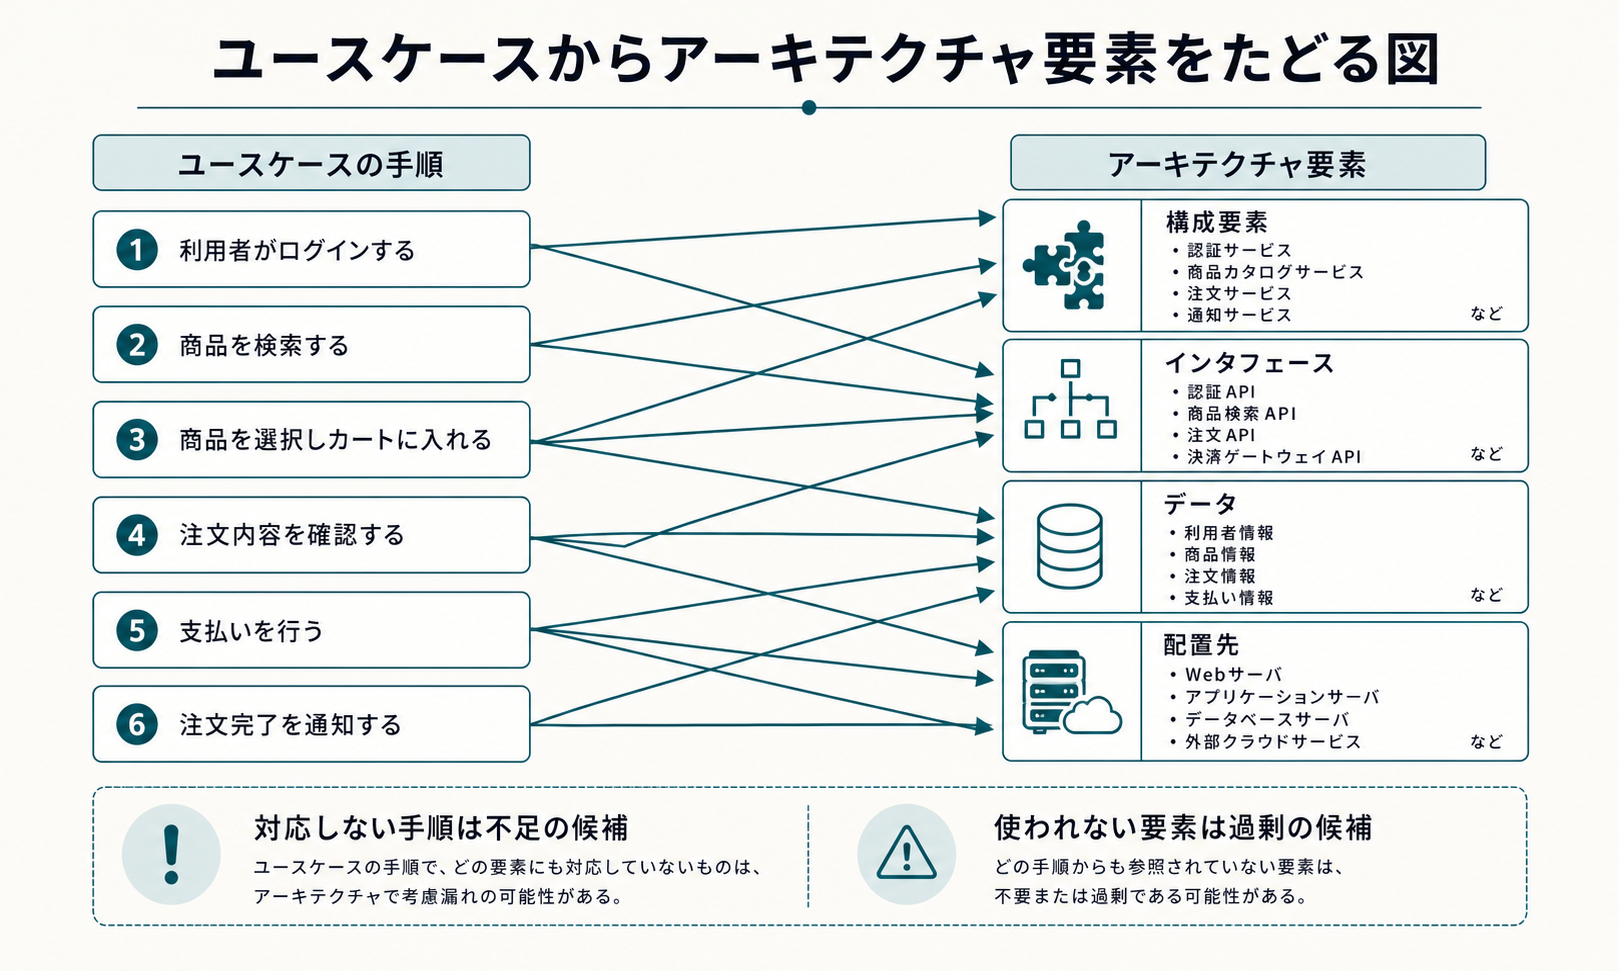
\includegraphics[width=0.96\linewidth]{assets/generated_figures/ch02/fig-ch02-08.png}}{\fbox{\parbox[c][48mm][c]{0.9\linewidth}{\centering 画像生成待ち\\ユースケースからアーキテクチャ要素をたどる図}}}
\par\smallskip
\refstepcounter{figure}\label{fig:ch02-08}図 \thefigure: ユースケースからアーキテクチャ要素をたどる図
\end{center}
図 \thefigure は、ユースケースからアーキテクチャ要素をたどる図を視覚的に整理したものである。
\par\smallskip

\subsubsection{アーキテクチャレビュー}
アーキテクチャレビューは、アーキテクチャの状態、品質、リスクを確認するための有効な方法である。レビューは、非公式な専門家レビューとして行われることもあれば、チェックリストに基づいて構造化されることもある。

より能動的なレビューでは、単に「この項目を確認したか」と聞くのではなく、レビュアが特定の活動を行って情報を得る。たとえば、「障害が発生したときに、どの構成要素がどの順で影響を受けるかを説明する」「利用者数が 10 倍になったときに、どの構成要素がボトルネックになるかを示す」といった活動である。

\par\smallskip\noindent\refstepcounter{table}\label{tab:ch02-06}表 \thetable: アーキテクチャレビューにおけるレビュー観点・確認すること\par\smallskip
表 \thetable は、アーキテクチャレビューにおけるレビュー観点・確認することを比較・確認しやすい形で整理したものである。\par\smallskip
\begin{longtable}{P{0.25\linewidth}P{0.67\linewidth}}
\toprule
レビュー観点 & 確認すること \\
\midrule
要求対応 & ASR に答える構成や判断があるか。 \\
品質特性 & 性能、可用性、変更容易性、安全性、セキュリティなどが説明されているか。 \\
トレードオフ & ある品質を優先したことで、別の品質にどのような影響があるか。 \\
\term{リスク}{Risk} & 未検証の前提、難しい技術、外部依存、単一障害点があるか。 \\
説明可能性 & 重要な意思決定に根拠が残っているか。 \\
実装適合性 & 実装がアーキテクチャに従っているか、または逸脱が管理されているか。 \\
\bottomrule
\end{longtable}

\subsubsection{アーキテクチャ測度}
\term{アーキテクチャ測度}{architecture metrics}とは、アーキテクチャの性質を数量で表すものである。測度は万能ではないが、複雑さ、依存関係、変更リスク、規約適合性を把握する手がかりになる。

代表的な測度には、構成要素間依存、循環依存、循環的複雑度、内部モジュール複雑度、結合度、凝集度、ネストの深さ、パターン・様式・API への準拠などがある。

継続的開発や DevOps の文脈では、アーキテクチャそのものではなく、アーキテクチャの状態を反映する過程測度も使われる。変更リードタイム、配置頻度、サービス復旧平均時間、変更失敗率などである。変更が遅く、復旧が難しく、失敗率が高い場合、アーキテクチャが変更や運用に適していない可能性がある。

\par\smallskip
\begin{center}
\centering
\IfFileExists{assets/generated_figures/ch02/fig-ch02-09.png}{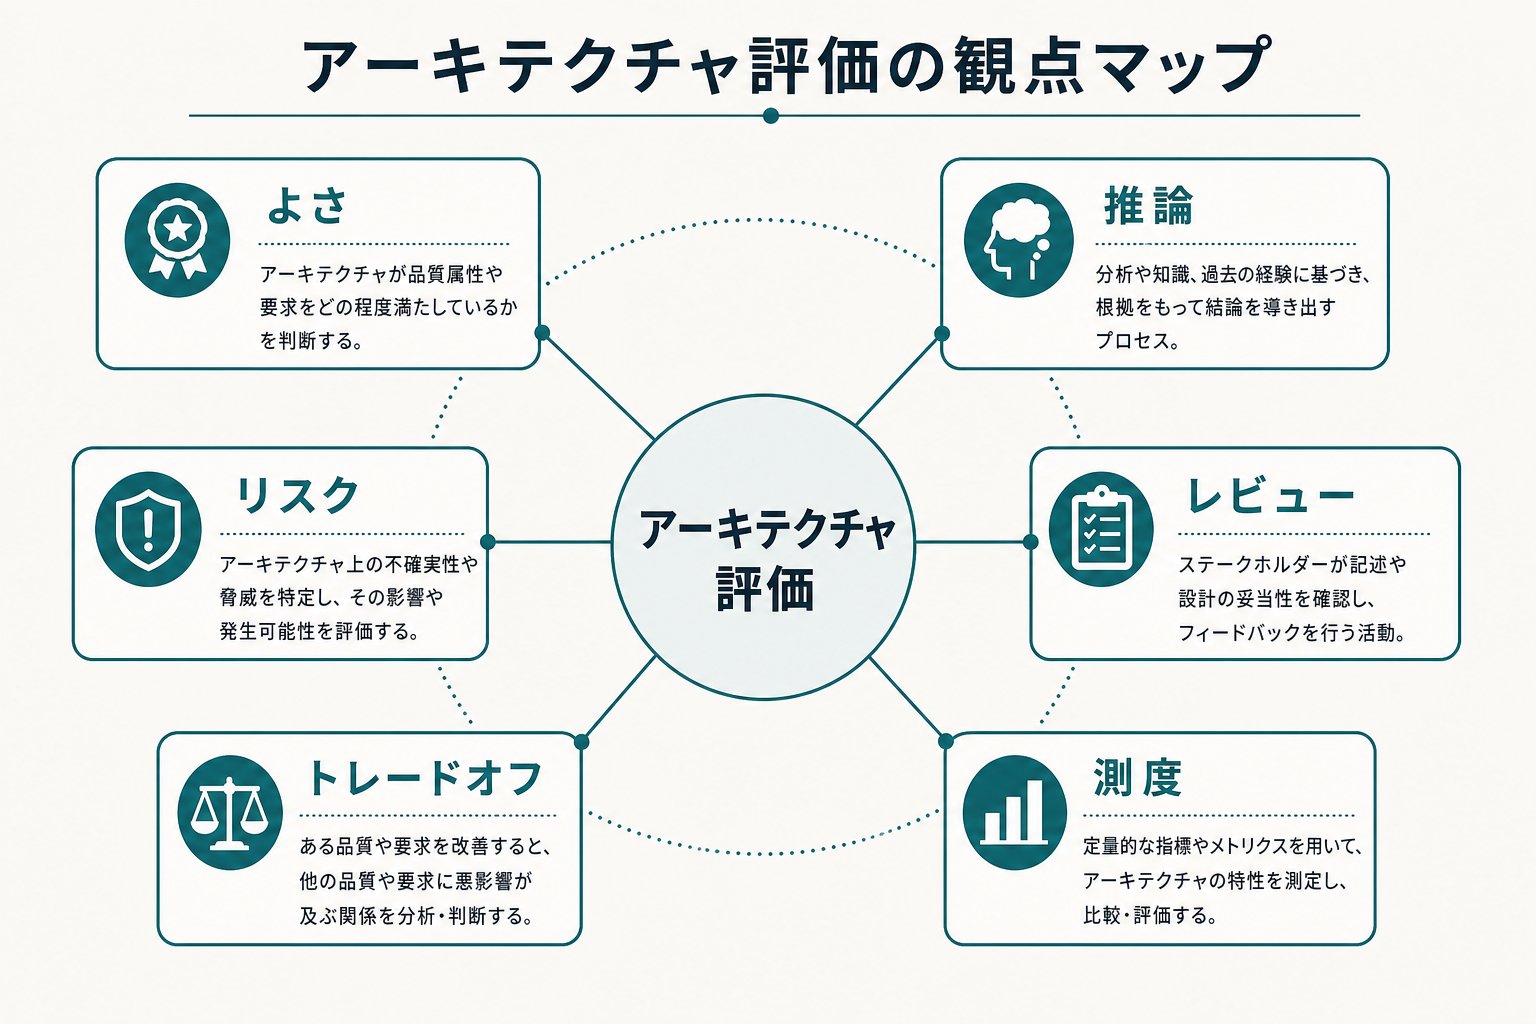
\includegraphics[width=0.96\linewidth]{assets/generated_figures/ch02/fig-ch02-09.png}}{\fbox{\parbox[c][48mm][c]{0.9\linewidth}{\centering 画像生成待ち\\アーキテクチャ評価の観点マップ}}}
\par\smallskip
\refstepcounter{figure}\label{fig:ch02-09}図 \thefigure: アーキテクチャ評価の観点マップ
\end{center}
図 \thefigure は、アーキテクチャ評価の観点マップを視覚的に整理したものである。
\par\smallskip
